\documentclass[11pt,letterpaper]{exam}
\usepackage[latin1]{inputenc}
\usepackage[left=3.00cm, right=3.00cm, top=3.00cm, bottom=3.00cm]{geometry}% You can change margins here
\usepackage{amsmath}
\usepackage{amsthm}
\usepackage[]{algorithm2e}
\usepackage{amssymb} % use for therefore
\usepackage{tabto}
\usepackage{gensymb}
\usepackage{graphicx} % resize table
\usepackage{listings}

\author{Elvric Trombert\\260673394\\Simon Zheng\\260744353}% Put your Student ID here
\title{Assignment 2 ECSE 420}
\date{October $10^{\textnormal{th}}$, 2018}
\begin{document}
	\maketitle
	\header{}{Assignment 2 ECSE 420}{}
	\hrulefill
	\begin{questions}
		\question
		\begin{parts}
			\part Answer coded in FilterLock.java
			\part
				Yes, filter lock allows overtaking another thread an arbitrary number of time. As mentioned in class it is possible that a thread stuck at a level, let's say level 1, may be taken over by another thread asking to enter the same critical section. Consider $t_i$ as being stuck at level 1, then the thread $t_j,t_k$ ask to acquire the lock as well, then $t_j$ sets itself as the victim for level 1, it allows $t_i$ to move up to the next level, but in our stimulation $t_i$ gets preempted straight after. Then, when $t_k$ sets itself as the victim for level 1, $t_j$ moves to the next level since $t_i$ was preempted. $t_j$ sets itself as the victim for level 2 before $t_i$ and so, when $t_i$ starts executing again, it gets stuck at level 2 by setting itself to be the victim of that level, allowing $t_j$ to move to the next level, overtaking $t_i$. If $t_i$ stays preempted, then it may be overtaken by an unlimited number of thread. Thus filter lock is not fair. 
			\part Answer coded in LamportBakeryLock.java	
			\part 
				No, the Bakery lock does not allow some Thread to take over other thread an arbitrary number of time as every time a Thread asks to enter the critical section it gets assigned a priority value (queue number). Hence a Thread that asks to access the critical section before another will have a lower queuing number which based on the while loop will make it access the critical section before any other thread with a higher number. Hence there can be no arbitrary taking over of threads with Bakery.
				
			\part
				To test the mutual exclusion we propose that we let different number of thread to increment a counter by 1. If at the end of the incrementation mutual exclusion indeed occur then the value of the counter should be equal to the number of thread that incremented it.
			\part The test where done in the class TestLocks.java\\
			Here is the sample output:
			\begin{lstlisting}
Testing FilterLock
The Lock worked successfully
Testing BakeryLock
The Lock worked successfully
			
Process finished with exit code 0
			\end{lstlisting}
		\end{parts}
		\question
		\begin{parts}
			\part
				LockOne: Regular register means that the old value can be read during an overlap between a read and a write. However a regular register will always read the current value if there is no overlap between a read and a write. In the case of LockOne we know that any thread will first have written to its flag before reading the flag of the other which implies that if Thread 0 enters the critical section it is either because Thread 1 has not written to its flag yet or is currently writing to it. Which means that when that given Thread 1 starts looking at Thread 0 flag, the write of Thread 0 will have already completed which means that it will read the newest value of the flag in this case true all the time until Thread 0 updates its flag again. Hence a regular register still achieves mutual exclusion.
			
			\part
				LockTwo: The same logic applies here as well when Thread 0 sets itself to the victim first it cannot enter the critical section, then when thread 1 sets itself to the victim thread 0 will enter the critical section, since thread 1 completed its write to victim, when reading its value directly after, it can no longer read the old value of victim (0 in this case) but must read the newest value (1 in this case) hence it will not enter the critical section. So mutual exclusion is still achieved.
		\end{parts}
		
		\question
		\begin{parts}
			\part
			True for 2 threads but not for $n>2$: assuming there are two threads A and B and that they are in the CS at the same time ($CS_A$ and $CS_B$).
			This implies that $busy == false$ as the only way to have passed the busy-waiting part is for the loop condition to have been false, which means $busy==false\ ||\ turn!=me$.
			It cannot have been $turn\ != me$.
			It can only ever be the turn of a single thread at any time.
			
			To enter the for loop a thread must have set $busy = true$ and this happens \textbf{after} the $turn = me$ as such if more than one thread are at the while-loop step, then all except the last to have set $turn = me$ will have $turn\ != me$ relative to them and we know they must have all set $busy = true$.
			
			This means that exactly one thread will proceed and unlock, so setting $busy = false$ to allow the thread whose $turn == me\ \&\&\ busy == true$ to proceed from the busy-wait.\newline
		
			Now for more than 2 threads this lock does not satisfy mutual: consider the following example: Thread1 calls the lock method first, so busy is true and turn equal 1 which is equal to Thread1 id. Hence that thread is suck in the while loop. 
			
			Thread2 comes in changing turn to 2 so Thread1 enters the critical section while Thread2 gets stuck in the while loop of the lock method.
			
			Then Thread3 comes in changing the turn variable to 3 which allows Thread2 to enter the critical section while Thread1 is still executing it. Hence at this step we no longer achieve mutual exclusion.
			
			\part
			This protocol is not deadlock free as if we have only 1 thread: Thread1 entering the lock method it will get stuck in the while loop and while no other thread comes along to change the value of turn it will remain stuck there which can cause a deadlock if it is the only thread running on the machine.
			
			\part
			Here we apply the same logic than above if only one thread Thread1 calls that lock method then it will remain stuck there while other thread may still run other methods but it will remain stuck and starve unless a second thread tries to access the same lock method on the same lock object.
		\end{parts}
		\newpage
		\question
		Fig 2, is sequentially consistent as we can have the following execution since we are allowed to execute different Thread methods at different times regardless of when they were called:
		\begin{figure}[h!]
			\centering
			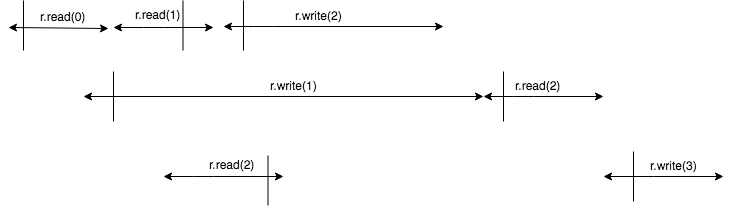
\includegraphics[scale=0.4]{Fig2Sequential}
		\end{figure}
		
		However Fig 2 is not linearizable as r.write(3) in thread C must happen before r.read(2) in thread B. Yet r.read(2) in thread C must happen before r.write(2) in thread A. Which forces the value read to be updated to 2 by thread A for thread C to read 2. At that point thread C has to write 3 before thread B can read 2 which makes it impossible for thread B to read 2.
		
		Fig3 can do neither of both as thread B writes 1 then read 2 and thread C writes 2 then reads 1. If thread B writes first then thread C has to overwrite the value with 2 before being able to read 1 and vice versa. Since they are no other threads that write anything but these two there is no possible arrangement that allow both threads to read the value shown on Fig3 hence we cannot make it sequentially consistent. If the execution is not sequentially consistent then it is also not linearizable either for the same reasons.
		
		\question
		\begin{parts}
			\part
				Yes the method reader could divide by 0. Since v is declared volatile it must be sequentially consistent. Hence when a thread accesses v it will always have the latest value however Java does not guarantee that non-volatile variable be sequentially consistent. Hence when the reader thread reads v==true then it may read x=0 when dividing as it may not be sequentially consistent. So the order would be write thread updates x then v, read thread reads v (which must be true as it is sequentially consistent) then the read thread reads x but the old value stored in cache not the newest value updated by v making it divide by 0.
			
			\part
				If they are both volatile then division by 0 cannot happen since each thread will always have the latest version of each variable value which means that when the reader thread enters the if (read v==true) then x would have had to already be updated to 42 in main memory and since it is volatile the reader thread will read the updated value.
				
				\quad If none of them are volatile then divide by 0 can occur as well for the same reason than in part (a) as Java does not guarantee sequential consistency for non-volatile variable the reader thread may read v as true and x as 0 during its execution.
		\end{parts} 
		
		\question
		\begin{parts}
			\part
				No its is not a regular M-valued MRSW register, as no matter where we write the new value the first bit $bit[0]$ will always be true making the reader thread always read $i=0$ (as we now write false to the right and not to the left in the array so true entries to the right are never changed to false) even when not reading concurrently with a write. Hence if we write true at byte $x=2$. Then the reader thread will never see it and keep reading $i=0$ even after the write operation finishes which is not regular as a read not overlapping with write should always read the newest value.
	
			\part
				The same argument holds for safe M-valued MRSW as even when the write method finishes after setting $x=2$ a reader thread will always read $i=0$ and never read the new value. Hence the register is not safe since safe register have to allow threads to read the new/correct value when the read does not overlap with a write.
		\end{parts} 
		
		\question
			Suppose we have a protocol that can solve binary consensus between two threads.
			Now, suppose we have $n$ threads, each labeled $t_1, t_2, ..., t_i, ..., t_n$.
			Then we simply use the protocol to solve binary consensus between $t_i$ and $t_j, \forall j \neq i$.
			
			So, for, say, 3 threads, if we lose a thread we still have 2 left with consensus and as such we have solved 2-thread binary consensus by doing so for $n$.
			Inductively, this works for any number $n$ greater than 2.
			
			Thus, if we cannot solve binary consensus for two threads, then we cannot for $n$ threads for $n>2$.
		\question
			If consensus over k values where $k>2$ for n threads was possible then we can implicitly get binary consensus. Consider consensus over $k=000$ where each 0 represent a bit. Then when getting consensus we can ignore that last 2 bits of k and just focus on the value taken by the first bit. In this case we have generated binary consensus as consensus can be achieved on k but the region of interest is just the first bit. Therefore if we can achieve consensus on $k$ where $k>2$ then we can get binary consensus as well by just accessing the value range we are interested in.
	\end{questions}

	\section*{Appendix}
	
	\subsection*{FilterLock.java}
	\begin{lstlisting}
package ca.mcgill.ecse420.a2;

import java.util.concurrent.TimeUnit;
import java.util.concurrent.locks.Condition;
import java.util.concurrent.locks.Lock;

public class FilterLock implements Lock {

  int numLevel;
  int[] level; // level[i] for thread i
  volatile int[] victim; // victim[L] for level L

  public FilterLock(int pNumLevel) {
    level = new int[pNumLevel];
    victim = new int[pNumLevel];
    for (int i = 0; i < pNumLevel; i++) {
      level[i] = 0;
    }
    numLevel = pNumLevel;
  }

  @Override
  public void lock() {
    int threadId = (int) (Thread.currentThread().getId() % numLevel);
    for (int L = 1; L < numLevel; L++) {
      level[threadId] = L;
      victim[L] = threadId;
      for (int j = 0; j < numLevel; j++) {
        while (j != threadId && level[j] >= L && victim[L] == threadId) {}
      }

      // One level at a time
      //      level[i] = L; // Announce intention to enter level L
      //      victim[L] = i; // Give priority to anyone but me
      //      while (/*(there exists k != i && level[k] >= L) && victim[L] == i*/) {} // Wait as
      // long as someone else is at same or higher level, and I'm designated victim. Thread enters
      // level L when it completes the loop
    }
  }

  @Override
  public void lockInterruptibly() throws InterruptedException {}

  @Override
  public boolean tryLock() {
    return false;
  }

  @Override
  public boolean tryLock(long time, TimeUnit unit) throws InterruptedException {
    return false;
  }

  @Override
  public void unlock() {
    int threadId = (int) (Thread.currentThread().getId() % numLevel);
    level[threadId] = 0;
  }

  @Override
  public Condition newCondition() {
    return null;
  }
}
	\end{lstlisting}
	
	\subsection*{LamportBakeryLock.java}
	\begin{lstlisting}
package ca.mcgill.ecse420.a2;

import java.util.Arrays;
import java.util.Collections;
import java.util.concurrent.TimeUnit;
import java.util.concurrent.atomic.AtomicInteger;
import java.util.concurrent.locks.Condition;
import java.util.concurrent.locks.Lock;

public class LamportBakeryLock implements Lock {

  boolean[] flag;
  volatile AtomicInteger[] label;
  int numLevel;

  public LamportBakeryLock(int n) {
    flag = new boolean[n];
    label = new AtomicInteger[n];
    for (int i = 0; i < n; i++) {
      flag[i] = false;
      label[i] = new AtomicInteger(0);
    }
    numLevel = n;
  }

  @Override
  public void lock() {
    int threadId = (int) (Thread.currentThread().getId() % numLevel);
    flag[threadId] = true;
//    label[threadId] = Collections.max(Arrays.asList(label)) + 1;
    // Find max manually to avoid certain runtime issues we got when testing the lock
    for (int i = 0; i < label.length; i++) {
      if (label[threadId].get() < label[i].get() && threadId != i) {
        label[threadId] = label[i];
      }
    }
    // ... + 1
    label[threadId].incrementAndGet();
    for (int i = 0; i < numLevel; i++) {
      while ((i != threadId)
          && flag[i]
          && ((label[i].get() < label[threadId].get()) || ((label[i] == label[threadId]) && i < threadId))) {}
    }

    //    flag[i] = true; // Doorway. true => I'm interested
    //    label[i] =  max(label[0], ...,label[n-1])+1; // Doorway. Take increasing label
    // (read labels in some arbitrary order)
    //    while (/*there exists k flag[k] && (label[i],i) > (label[k],k)*/); // Someone is
    // interested
    // whose (label,i) in lexicographic order is lower
  }

  @Override
  public void lockInterruptibly() throws InterruptedException {}

  @Override
  public boolean tryLock() {
    return false;
  }

  @Override
  public boolean tryLock(long time, TimeUnit unit) throws InterruptedException {
    return false;
  }

  @Override
  public void unlock() {
    int threadId = (int) (Thread.currentThread().getId() % numLevel);
    flag[threadId] = false;
  }

  @Override
  public Condition newCondition() {
    return null;
  }
}
	\end{lstlisting}
\subsection*{TestLocks.java}
\begin{lstlisting}
package ca.mcgill.ecse420.a2;

import java.util.concurrent.TimeUnit;
import java.util.concurrent.locks.Condition;
import java.util.concurrent.locks.Lock;

public class FilterLock implements Lock {

  int numLevel;
  int[] level; // level[i] for thread i
  volatile int[] victim; // victim[L] for level L

  public FilterLock(int pNumLevel) {
    level = new int[pNumLevel];
    victim = new int[pNumLevel];
    for (int i = 0; i < pNumLevel; i++) {
      level[i] = 0;
    }
    numLevel = pNumLevel;
  }

  @Override
  public void lock() {
    int threadId = (int) (Thread.currentThread().getId() % numLevel);
    for (int L = 1; L < numLevel; L++) {
      level[threadId] = L;
      victim[L] = threadId;
      for (int j = 0; j < numLevel; j++) {
        while (j != threadId && level[j] >= L && victim[L] == threadId) {}
      }

      // One level at a time
      //      level[i] = L; // Announce intention to enter level L
      //      victim[L] = i; // Give priority to anyone but me
      //      while (/*(there exists k != i && level[k] >= L) && victim[L] == i*/) {} // Wait as
      // long as someone else is at same or higher level, and I'm designated victim. Thread enters
      // level L when it completes the loop
    }
  }

  @Override
  public void lockInterruptibly() throws InterruptedException {}

  @Override
  public boolean tryLock() {
    return false;
  }

  @Override
  public boolean tryLock(long time, TimeUnit unit) throws InterruptedException {
    return false;
  }

  @Override
  public void unlock() {
    int threadId = (int) (Thread.currentThread().getId() % numLevel);
    level[threadId] = 0;
  }

  @Override
  public Condition newCondition() {
    return null;
  }
}
\end{lstlisting}
\end{document}